\documentclass[11pt,a4paper]{article}

\usepackage{german,anysize,amsmath,amssymb,amsthm,paralist,array}
\usepackage{url}
\usepackage{graphicx}

\selectlanguage{german}

\pagestyle{empty}

\setlength{\textheight}{27cm}
\setlength{\parindent}{0cm}


\begin{document}
\textsc{Technische Universit"at Berlin}{\small\hfill 
Scalable Data Mining and Data Analysis}\\
{\small Database Systems and Information Management Group}

\bigskip
\centerline{\Large\textbf{Assignment}}
\centerline{\emph{Graph Mining with Stratosphere}}
\bigskip

In this assignment, you will use the Stratosphere system (\url{http://www.stratosphere.eu/}) for conducting network analysis. You will analyze the ``Slashdot-Zoo'' dataset, the signed social network of users of the technology news site Slashdot (\url{http://slashdot.org}), connected by directed `friend' and `foe' relations. The network contains 79,120 vertices connected by 515,581 edges. Every edge is marked with either `+1' or `-1' to denote a friend or foe relationship. 

\bigskip
\centerline{\textbf{Preparation}}

\begin{itemize}
	\item Clone the source code for the assignment from \url{https://github.com/stratosphere/graphmining-tutorial}. It is a standard Java project than can be built with Maven.

	\item Download the dataset from \url{http://konect.uni-koblenz.de/networks/slashdot-zoo} and unpack it on your machine.

	\item Adjust the method \textit{de.tuberlin.dima.aim3.graphmining.Config\#pathToSlashdotZoo()} to point to the location of the file \textit{out.slashdot-zoo} that you unpacked from the downloaded dataset.

\bigskip
\bigskip
\bigskip
\centerline{\textbf{Network Statistics}}
\bigskip

The first part of the assignment deals with the computation of simple network statistics such as the distribution of the number of out-going edges per vertex. 

The class \textit{de.tuberlin.dima.aim3.graphmining.statistics.OutDegreeDistribution} describes a Stratosphere program which computes this distribution. Note that it ignores the sign of the edges.

\begin{enumerate}

\item \textbf{Signed out-degree distribution}

Write a new Stratosphere program \textit{SignedOutDegreeDistribution} which computes two out-degree distributions, the first one incorporating only friend edges, the second one incorporating only foe edges.

\item \textbf{Determining the average ratio of friends and foes}

Write a new Stratosphere program \textit{AverageFriendFoeRatio} that computes the average ratio of friends and foes per vertex in the network. Note that you can create a \textit{ReduceStub} without \textit{keyField} as a way to compute the final aggregate number for this task.
 
\newpage
\centerline{\textbf{Simulating Message Spread in Networks}}

In this exercise, you will use the iterative data flows provided by Stratosphere to simulate message spread in networks. 

The underlying algorithm aims to simulate the forwarding of a chain-letter between users in the social network. Initially, a tiny fraction of the users is selected as initiators of the chain-letter. For each user that they have a connection to, they will forward the letter with a probability of 50\%. All users that now receive the letter (and have not seen it yet) will repeat this process: They will forward the letter again to their connections with a probability of 50\% per link.

The class \textit{de.tuberlin.dima.aim3.graphmining.chainletter.ChainLetter} has a preliminary implementation of this algorithm. The following diagram describes the dataflow in this iterative Stratosphere program:

	\begin{figure}[h]
		\begin{center}
			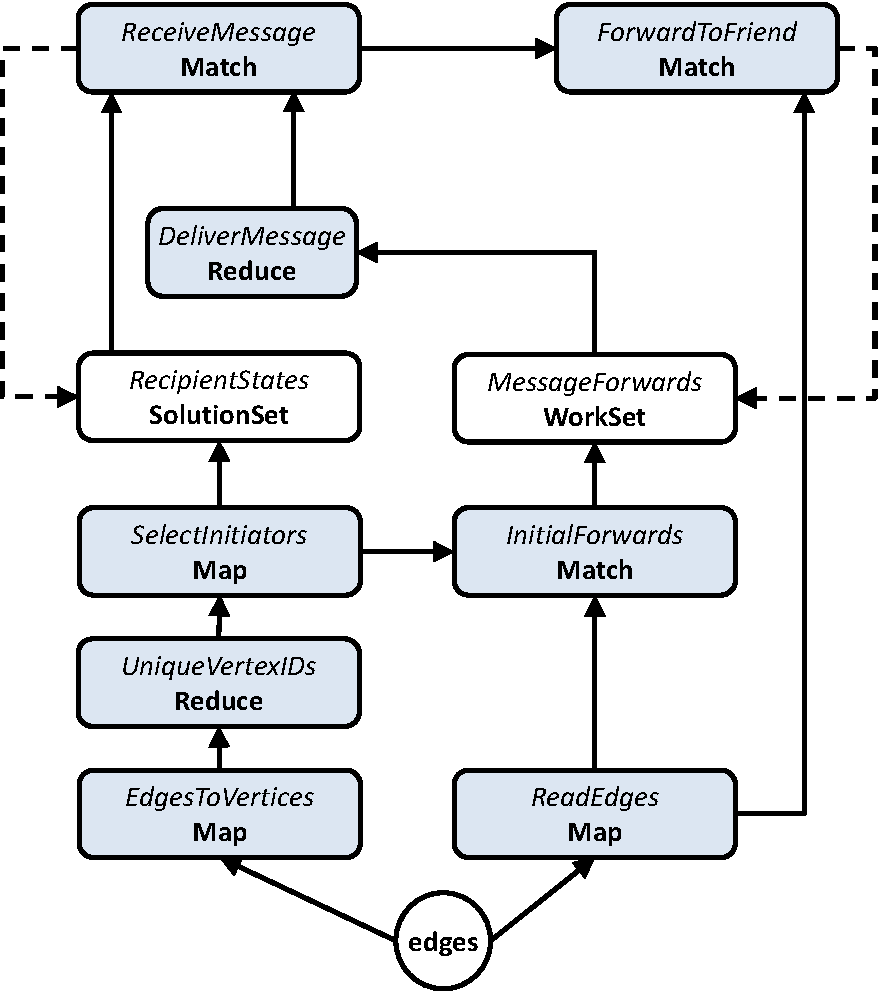
\includegraphics[scale=0.5]{chainletter-plan-crop.pdf}
		\end{center}
	\end{figure}


\item \textbf{Understand the dataflow}

For every operator used in the plan, describe its role in the simulation algorithm in 1 or 2 short sentences. Why is this algorithm implementation guaranteed to convergence?

\item \textbf{Join performance}

Look at the join performed by the \textit{InitialForwards}-operator. What kind of join is it? How could you alter the plan to increase the performance for this join?

\item \textbf{Messages to friends only}

Modify the code to ensure that messages are only forwarded between friends.



\end{enumerate}

\end{document}
